% begin module improper-integral-type1-ex1
\begin{frame}
\begin{example} %[Example 1, p. 545]
Determine whether $\int_1^\infty \frac{1}{x} \diff x$ is convergent or divergent.
\begin{columns}[c]
\column{.4\textwidth}


\psset{xunit=1cm, yunit=1cm}
\begin{pspicture}(-0.4, -0.4)(3.4,2.2) 
\psframe*[linecolor=white](-0.4,-0.4)(3.4,2.2) 
\tiny 

\pscustom*[linecolor=cyan]{
%Function formula: x^{-1} 

\psplot[linecolor=\psColorGraph, plotpoints=1000]{1.000000}{3.000000}{x -1.0000000 exp }\psline(3.000000, 0)(1.000000, 0)}

%Function formula: x^{-1} 

\psplot[linecolor=\psColorGraph, plotpoints=1000]{0.5}{3.000000}{x -1.0000000 exp }
\psaxesStandard{-0.40}{-0.4}{3.3}{2}
\rput(1.5, 1.5){$y=\frac{1}{x}$}
\end{pspicture} 
%\ 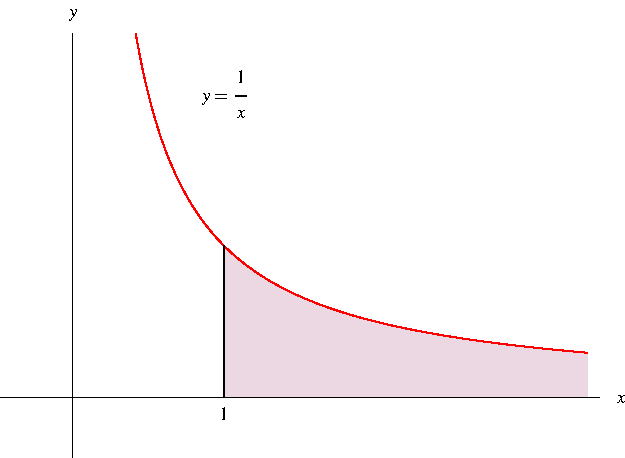
\includegraphics[height=3cm]{improper-integrals/pictures/08-08-ex1b.pdf}%

%\begin{center}
\uncover<7->{Infinite area}%
%\end{center}

\ \uncover<8->{%
\psset{xunit=1cm, yunit=1cm}
\begin{pspicture}(-0.4, -0.4)(3.3,2.2) 
\psframe*[linecolor=white](-0.4,-0.4)(3.3,2.2) 
\tiny 
\pscustom*[linecolor=cyan]{
%Function formula: x^{-2} 

\psplot[linecolor=\psColorGraph, plotpoints=1000]{1.000000}{3.000000}{x -2.0000000 exp }\psline(3.000000, 0)(1.000000, 0)}

%Function formula: x^{-2} 

\psplot[linecolor=\psColorGraph, plotpoints=1000]{0.75}{3.000000}{x -2.0000000 exp }
\psaxesStandard{-0.400000}{-0.4}{3.200000}{2}
\rput(1.5, 1.5){$y=\frac{1}{x^2}$}

\end{pspicture} 

%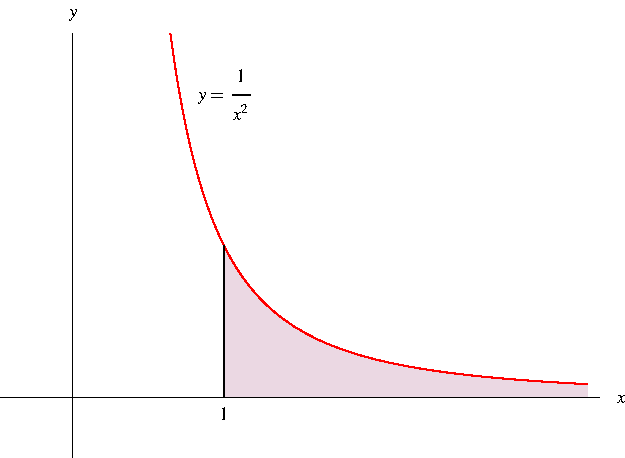
\includegraphics[height=3cm]{improper-integrals/pictures/08-08-ex1a.pdf}%
}%

%\begin{center}
\uncover<8->{Finite area}%
%\end{center}
\column{.6\textwidth}
\begin{eqnarray*}
\uncover<2->{%
\int_1^\infty \frac{1}{x}\diff x%
}%
& \uncover<2->{ = } & %
\uncover<2->{%
\lim_{t\rightarrow \infty} \int_1^t \frac{1}{x}\diff x%
}\\%
& \uncover<3->{ = } & %
\uncover<3->{%
\lim_{t\rightarrow \infty} \left[ \ln x\right]_1^t%
}\\%
& \uncover<4->{ = } & %
\uncover<4->{%
\lim_{t\rightarrow \infty} (\ln t - \ln 1)%
}\\%
& \uncover<5->{ = } & %
\uncover<5->{%
\lim_{t\rightarrow \infty} \ln t%
}%
\uncover<6->{ = \infty }%
\end{eqnarray*}
\uncover<7->{Therefore the improper integral is divergent.}
\end{columns}
\end{example}
\end{frame}
% end module improper-integral-type1-ex1
